%%%%%%%%%%%%%%%%%%%%%%%%%%%%%%%%%%%%%%%%%%%%%%%%%%%%%%%%%%%%%%%%%%%%%%%%%%%%%%%%
%2345678901234567890123456789012345678901234567890123456789012345678901234567890
%        1         2         3         4         5         6         7         8

\documentclass[letterpaper, 10 pt, conference]{ieeeconf}  % Comment this line out if you need a4paper

%\documentclass[a4paper, 10pt, conference]{ieeeconf}      % Use this line for a4 paper

\IEEEoverridecommandlockouts                              % This command is only needed if 
                                                          % you want to use the \thanks command

\overrideIEEEmargins                                      % Needed to meet printer requirements.

% See the \addtolength command later in the file to balance the column lengths
% on the last page of the document

% The following packages can be found on http:\\www.ctan.org
%\usepackage{graphics} % for pdf, bitmapped graphics files
%\usepackage{epsfig} % for postscript graphics files
%\usepackage{mathptmx} % assumes new font selection scheme installed
%\usepackage{times} % assumes new font selection scheme installed
%\usepackage{amsmath} % assumes amsmath package installed
%\usepackage{amssymb}  % assumes amsmath package installed
\usepackage{gensymb}
\usepackage{graphicx}
\usepackage{import}
\graphicspath{ {images/} }
\maxdeadcycles=1000
\setlength{\tabcolsep}{3pt}

\title{\LARGE \bf
High-Fidelity Simulation for Evaluating Robotic Vision Performance
}


\author{John Skinner$^{1}$, Sourav Garg$^{1}$, Niko Suenderhauf$^{1}$, Peter Corke$^{1}$, Ben Upcroft$^{1}$, Michael Milford$^{1}$% <-this % stops a space
\thanks{$^{1}$ Australian Centre for Robotic Vision,
        Queensland University of Technology,
        2 George St, Brisbane, Australia}%
%        {\tt\small jr.skinner@hdr.qut.edu.au}
%        {\tt\small sourav.garg@hdr.qut.edu.au}
%        {\tt\small niko.suenderhauf@qut.edu.au}
%        {\tt\small peter.corke@qut.edu.au}
%        {\tt\small ben.upcroft@qut.edu.au}
%        {\tt\small michael.milford@qut.edu.au}
}


\begin{document}



\maketitle
\thispagestyle{empty}
\pagestyle{empty}


%%%%%%%%%%%%%%%%%%%%%%%%%%%%%%%%%%%%%%%%%%%%%%%%%%%%%%%%%%%%%%%%%%%%%%%%%%%%%%%%
\begin{abstract}

\import{./}{abstract.tex}

\end{abstract}


%%%%%%%%%%%%%%%%%%%%%%%%%%%%%%%%%%%%%%%%%%%%%%%%%%%%%%%%%%%%%%%%%%%%%%%%%%%%%%%%
\section{INTRODUCTION} \label{sec:introduction}

\import{./}{introduction.tex}

\begin{figure*}[t]
    \centering
    \includegraphics[width=\textwidth]{street-scene-overview-dataset-examples}
    \caption{The street scene used to capture the image datasets that were used for testing the place recognition algorithms. The line of white dots shows the baseline path followed by the camera when generating the datasets to test Sum of Absolute Differences matching and SeqSLAM. OrbSLAM test datasets follow a slightly different path so that they can loop their way around and end where they started.}
    \label{fig:street-scene-overview}
\end{figure*}

\section{PRIOR RESEARCH} \label{sec:prior-research}

\import{./}{prior-research.tex}

\section{ANALYSIS OF PLACE RECOGNITION} \label{sec:analysis-place-rec}

\begin{figure*}[t]
    \centering
    \includegraphics[width=16cm]{data-comparison-stacked}
    \caption{A Sample of the variation found in the datasets used for testing. The first row shows lateral offset, from left to right, images are offset are left 3.5m, 2m, 1m, 0.4m, 0.2m, Then the baseline, then offset right 0.2m, 0.4m, 1m, 2m, and 3.5m. The second row shows vertical orientation change,  left to right, images are angled are up $30\degree$, $15\degree$, $10\degree$, $5\degree$, Then the baseline, then angled down $5\degree$, $10\degree$, $15\degree$, and $30\degree$. The third row shows horizontal orientation change, from left to right, images are angled are left $30\degree$, $15\degree$, $10\degree$, $5\degree$, Then the baseline, then angled right$5\degree$, $10\degree$, $15\degree$, and $30\degree$. Finally, the lowest row shows samples of time of day variation, from left to right, images are taken at dawn, in the morning, at noon, in the afternoon, and at sunset.}
    \label{fig:dataset-example}
\end{figure*}

%\begin{figure*}[t]
%    \includegraphics[width=16cm,height=2cm]{lateral-offset-comparison}
%    \caption{Sample images used to test lateral offset viewpoint invariance. From left to right, images are offset are left $3.5m$, $2m$, $1m$, $0.4m$, $0.2m$, Then the baseline, then offset right $0.2m$, $0.4m$, $1m$, $2m$, and $3.5m$}
%    \label{fig:dataset-offset-example}
%\end{figure*}
%
%\begin{figure*}[t]
%    \includegraphics[width=16cm]{vertical-orientation-change-comparison}
%    \caption{Sample images used to test orientation viewpoint invariance. From left to right, images are angled are up $30\degree$, $15\degree$, $10\degree$, $5\degree$, Then the baseline, then angled down $5\degree$, $10\degree$, $15\degree$, and $30\degree$}
%    \label{fig:dataset-pitch-example}
%\end{figure*}
%
%\begin{figure*}[t]
%    \includegraphics[width=16cm,height=2cm]{horizontal-orientation-change-comparison}
%    \caption{Sample images used to test orientation viewpoint invariance. From left to right, images are angled are left $30\degree$, $15\degree$, $10\degree$, $5\degree$, Then the baseline, then angled right$5\degree$, $10\degree$, $15\degree$, and $30\degree$}
%    \label{fig:dataset-yaw-example}
%\end{figure*}
%
%\begin{figure*}[t]
%    \includegraphics[width=16cm,height=2cm]{time-of-day-comparison}
%    \caption{Sample images used to test condition invariance. From left to right, images are taken at dawn, in the morning, at noon, in the afternoon, and at sunset}
%    \label{fig:dataset-time-of-day-example}
%\end{figure*}

To demonstrate the effectiveness of high-fidelity simulation as an analysis tool for computer vision, we performed an in depth analysis of the viewpoint and time-of-day invariance of two different state-of-the-art place recognition algorithms, SeqSLAM \cite{Milford2012} and OrbSLAM \cite{Montiel2015}. Then, to demonstrate the versatility of we performed an analysis of the viewpoint dependence of object recognition.

\subsection{Simulation Setup: Unreal Engine 4}

The simulation tool used in this paper was the Unreal Engine 4, developed by Epic Games Inc.

All of the test images used were generated from the same street scene, shown in Figure \ref{fig:street-scene-overview}. The 3D models used were either sourced for free from TurboSquid (www.turbosquid.com), with significant manual clean up, or were produced manually. The landscape was produced using the basic version of WorldMachine (http://www.world-machine.com). All lighting is as computed by the Unreal Engine, using standard sky and light assets provided with the engine.

To generate the image data, the camera was made to move along a specified path and produce images at fixed intervals.
The simulator allows us to precisely repeat the same path, and introduce calculated and precise variations upon it.
In order to explore how the performance of place recognition changes with time of day and viewpoint change, passes along the path were generated for 5 different times of day in combination with increasing lateral offsets or camera tilts (Figure \ref{fig:dataset-example}).

%\begin{figure}[t]
%    \includegraphics[width=8cm]{dataset-image-variety-grid}
%    \caption{Sample images from the datasets used, all images are taken from the same place at different times of day and viewpoint variations. From left to right, viewpoints are the base unmodified path, offset left 2m, offset right 2m, angled up $30\degree$, and angled right $30\degree$}
%    \label{fig:dataset-example}
%\end{figure}

\subsection{Place Recognition: Sum of Absolute Differences}

The first test we did was on simple place recognition using simple sum-of-absolute-differences (SAD) based image matching. While this is neither state-of-the-art nor particularly effective, sum-of-absolute-differences is a common metric which is used in many computer vision algorithms, including SeqSLAM discussed below. As such, an analysis of its performance characteristics is potentially interesting.

Before matching, each image is down-sampled to 64x64 pixels and reduced to greyscale, in order to save computation time. The matcher used compares each image in a query dataset to each of those in a reference dataset, and considers the reference image with the lowest sum of absolute difference to be a match. The performance is then the percentage of images for which the matched reference image is taken from a place close to the query image.

The matcher is tested using 130 different combinations of time of day and viewpoint changes, so that we can see how the performance falls off as both increase. The results are summarized in Figure \ref{fig:sad-results-stacked}.

Figure \ref{fig:sad-results-stacked} shows that SAD-based matching seems to be relatively robust against small lateral offsets, falling of after approximately $2m$. There is similar falloff as time of day approaches sunrise or sunset, and seems to be relatively symmetrical. The small number of samples makes this change seem relatively smooth, but it also seems plausible that it may instead change rapidly around dawn and sunset when the lighting change has the most effect. Resolving this is simply a matter of sampling the distribution further.

Interestingly, matching rate falls off similarly with angle change irrespective of the direction of change (compare the lower two plots in Figure \ref{fig:sad-results-stacked}). Matching performance seems to follow an exponential decay with angle, but additional sampling would need to be performed to verify that hypothesis. It may also be worth investigating the effects of multiple orientation offsets combined together to see how they compound. Were it the aim of this paper, it would be relatively simple to generate additional required sample passes to properly evaluate, but it is beyond the current scope.

\begin{figure}[ht]
    \centering
    \includegraphics[width=7cm]{SAD-results-stacked}
    \caption{Match percentage for Sum of Absolute Differences for, from top to bottom, lateral offset, vertical orientation change (pitch), and lateral orientation change (yaw). Each offset was tested across several times of day.}
    \label{fig:sad-results-stacked}
\end{figure}

%\begin{figure}[h]
%    \includegraphics[width=8cm]{SAD-matching-performance-over-lateral-offset-and-time-of-day}
%    \caption{Sum of absolute difference matching over both time of day and lateral offset change.}
%    \label{fig:sad-results-stacked}
%\end{figure}

%\begin{figure}[h]
%    \includegraphics[width=8cm]{SAD-matching-performance-over-vertical-orientation-change-and-time-of-day}
%    \caption{Sum of absolute difference match rate over both time of day and vertical orientation change}
%    \label{fig:sad-results-pitch}
%\end{figure}

%\begin{figure}[h]
%    \includegraphics[width=8cm]{SAD-matching-performance-over-lateral-orientation-change-and-time-of-day}
%    \caption{Sum of absolute difference match rate over both time of day and lateral offset change}
%    \label{fig:sad-results-yaw}
%\end{figure}

\subsection{Place Recognition: SeqSLAM}

The first full place recognition algorithm we investigated was SeqSLAM, first described by Milford and Wyeth \cite{Milford2012}. SeqSLAM is a place recognition algorithm that searches for loop closures by attempting to match sequences of similar images. It measures image similarity using sum of absolute differences as analysed in the previous section.

To perform the test, we generated 130 passes across 5 times of day and 26 different viewpoint variations from the street scene used in the other tests (figure \ref{fig:dataset-example}. We chose the baseline pass at noon as the reference dataset, and compared it to all 130 of the other datasets (including itself). For each dataset we calculated the maximum F1 score, the results are summarized in Figure \ref{fig:seqslam-results-stacked}.

The first immediately obvious result is the anomalous low performance values for a left 0.2m offset in the morning and at sunset, and the low performance across all times of day at a 10\degree vertical orientation change.  All of these changes are sudden and extreme, so the initial inclination is to sample around these points to see if there is a smooth or sudden decline. Based on the results of tweaking the parameters however, it seems more likely that SeqSLAM performance is sensitive to having achieved a certain level of matching, and that it will either perform very well or badly, rather than smoothly transition.

The other feature of note in the performance characteristics is the way the F1 score plateaus for translational offsets of less than 1 and orientation changes of 5\degree. When the algorithm performs well, it seems to do so irrespective of the time of day. Strong condition invariance has been noted in previous work as a particular feature of SeqSLAM \cite{Milford2012}, so it is good to see it confirmed here. Note however that when the performance falls off, it becomes less condition invariant, falling off further toward sunset and sunrise.

Using high-fidelity simulation has allowed us to explore the behaviour of SeqSLAM more comprehensively than ever before, and has revealed new details of its behaviour. Further investigation will be required to find the reason for this, which will lead to it becoming more reliable and even more robust.

\begin{figure}[t]
    \centering
    \includegraphics[width=7cm]{SeqSLAM-results-stacked}
    \caption{SeqSLAM performance over, from top to bottom, lateral offset, vertical orientation change (pitch), and horizontal orientation change (yaw). Each viewpoint change is captured over 5 times of day to show how performance degrades over both viewpoint and condition change}
    \label{fig:seqslam-results-stacked}
\end{figure}

%\begin{figure}[t]
%    \includegraphics[width=8cm]{SeqSLAM-results-offset}
%    \caption{SeqSLAM fscore over both time of day and lateral offset change}
%    \label{fig:seqslam-results-offset}
%\end{figure}

%\begin{figure}[t]
%    \includegraphics[width=8cm]{SeqSLAM-results-pitch}
%    \caption{SeqSLAM fscore over both time of day and lateral offset change}
%    \label{fig:seqslam-results-pitch}
%\end{figure}

%\begin{figure}[t]
%    \includegraphics[width=8cm]{SeqSLAM-results-yaw}
%    \caption{SeqSLAM fscore over both time of day and lateral offset change}
%    \label{fig:seqslam-results-yaw}
%\end{figure}

\subsection{Visual SLAM: ORB-SLAM}

The second algorithm tested was ORB-SLAM \cite{Montiel2015}. ORB-SLAM is a feature-based monocular SLAM system, that performs feature-based visual feature tracking, place recognition, mapping and loop closure using ORB features.

To test OrbSLAM, we again generated a variety of image datasets from the same street scene, with 5 different times of day, a baseline pass and 20 different viewpoint variations. Due to the mapping element of OrbSLAM, all datasets were made to start and end in the same place. To test the performance, each of the datasets was appended to the noon baseline dataset (acting as a reference pass), and camera trajectories were generated. These trajectories were then compared with the ground truth to calculate the Absolute Trajectory Error after aligning their scale. Results are summarised in Figure \ref{fig:orbslam-results-stacked}.

The observed performance of ORB-SLAM is patchy, error seems to range inconsistently, irrespective of the viewpoint or conditions. Even the baseline datasets with no viewpoint change between the passes have trouble sometimes, such as in the morning pass. On the other hand, the performance of the algorithm doesn't seem to depend on viewpoint or time of day at all, but on other factors not controlled in our data. In the end, the inconsistent performance of ORB-SLAM under comprehensive testing is a question for the developers.

\begin{figure}[t]
    \centering
    \includegraphics[width=7cm]{orbslam-results-stacked}
   \caption{ORB-SLAM average trajectory error over, from top to bottom, lateral offset, vertical orientation change (pitch), and horizontal orientation change (yaw). Each viewpoint change is captured for 5 different times of day.}
    \label{fig:orbslam-results-stacked}
\end{figure}

%\begin{figure}[t]
%    \includegraphics[width=8cm]{orbslam-results-stacked}
%    \caption{OrbSLAM average trajectory error over both time of day and lateral offset change}
%    \label{fig:orbslam-results-offset}
%\end{figure}
%
%\begin{figure}[t]
%    \includegraphics[width=8cm]{orbslam-pitch-results}
%    \caption{OrbSLAM average trajectory error over both time of day and lateral offset change}
%    \label{fig:orbslam-results-pitch}
%\end{figure}
%
%\begin{figure}[t]
%    \includegraphics[width=8cm]{orbslam-yaw-results}
%    \caption{OrbSLAM average trajectory error over both time of day and lateral offset change}
%    \label{fig:orbslam-results-yaw}
%\end{figure}

\subsection{SeqSLAM parameter tuning}

The detailed analysis we have performed can be used to inform subsequent actions, including parameter tuning. To demonstrate this, we again tested the performance of Sum of Absolute Differences on the noon datasets across the range of lateral offsets shown in Figure \ref{fig:dataset-example} with a variety of different offset window parameters. SeqSLAM uses Sum of Absolute Differences combined with an offset window parameter that shifts the image pixels to achieve a better matching image. The results of this test can be seen in Figure \ref{fig:offset-matching-param-results}.

This data suggests that for distances up to 3.5m offset from the reference location, it is best to use the smaller 4 pixel window range. The use of an offset window shows clear improvement in performance, but larger windows may  introduce false matches. Larger windows may be appropriate to larger offset, and if necessary we could easily have tested this by generating more data and extending the experiment.

\begin{figure}[t]
    \centering
    \includegraphics[width=7cm]{offset-matching-results}
    \caption{Sum of Absolute Difference matching rate as the maximum offset window is increased. This result helps us choose a maximum offset appropriate for a given lateral offset}
    \label{fig:offset-matching-param-results}
\end{figure}

\textbf{Benefits of Simulation:} The performance curves generated using simulated datasets for SeqSLAM show a peculiar behaviour for certain parameter values. This enables a comprehensive evaluation of the algorithm for such cases which is not expected in general. The corresponding input parameters of SeqSLAM which might have caused the unexpected intermittent performance drop as shown in the Figure \ref{fig:seqslam-results-stacked} could be the \emph{Offset Matching Range} and/or \emph{Patch Normalization} factor. We further analysed the performance drop for different times of day at $10\degree$ pitch. Figure \ref{fig:seqSLAM-diffMat} shows the SAD matrix comparison with ground truth, true positives and false positives marked.

\begin{figure*}[t]
\centering
\begin{tabular}[t]{ccccccccc}
    \includegraphics[scale=0.2]{1-down30} &
    \includegraphics[scale=0.2]{2-down15} &
    \includegraphics[scale=0.2]{3-down10} &
    \includegraphics[scale=0.2]{4-down5} &
    \includegraphics[scale=0.2]{5-base} & 
    \includegraphics[scale=0.2]{6-up5} &
    \includegraphics[scale=0.2]{7-up10} &
    \includegraphics[scale=0.2]{8-up15} &
    \includegraphics[scale=0.2]{9-up30} \\
    Down $30\degree$ & Down $15\degree$ & Down $10\degree$ & Down $5\degree$ &
    Baseline &
    Up $5\degree$ & Up $10\degree$ & Up $15\degree$ & Up $30\degree$

\end{tabular}
    \caption{The SAD matrix for comparison of Noon Baseline dataset with a change in orientation of camera's pitch. The ground truth is marked in blue and forms the diagonal of the matrix with true positives overlaid in yellow on the diagonal. The false positives are marked in red.}
    \label{fig:seqSLAM-diffMat}
\end{figure*}

\subsection{Comparison to real-world}

It is important to verify that performance change in simulation is representative of performance change in the real world. To test this, we compared performance drop over lateral viewpoint change using SeqSLAM for data from a real street and for data generated from a simulation of a similar street. The real data experiment images are shown in Figure \ref{fig:real-world-data} and the performance results can be seen in Figure \ref{fig:real-world-results}.

\begin{figure*}[t]
\centering
    \includegraphics[width=15cm,height=2cm]{real-data-lateralOffset} \\
    \vspace{0.1cm}
    \includegraphics[width=15cm,height=2cm]{simulated-data-lateralOffset}
    \caption{Images for five different traversals of a street with different lateral offsets. This real world data (top) is used to compare the trend of performance change with change in lateral shifts as compared to the simulated data (bottom).}
    \label{fig:real-world-data}
\end{figure*}

Unsurprisingly, observed performance is consistently better in simulation; we ascribe this to a lack of sufficient realism in the simulation, which was built simply and quickly. However, the performance follows the same trends in both environments, falling off smoothly as the offset difference increases. This demonstrates that performance results obtained in simulation obey similar trends to data obtained from even simplistic simulations.

\begin{figure}[t]
    \centering
    \includegraphics[width=7cm]{real-world-results}
    \caption{Comparison of SeqSLAM performance falloff between simulated and real-world environments as lateral offset increases. As is often the case, simulated performance is better in an absolute sense, but the trend is the same in both cases. This data was not compared across multiple times of day.}
    \label{fig:real-world-results}
\end{figure}

%\section{RESULTS}

% TODO: I don't think this section exists explicitly, I'm keeping it for notes
%contributions streams throughout the paper

%\begin{enumerate}
%    \item simulation as a useful tool
%    \item closing the loop - redoing based on automated triggers (not enough resolution)
%    \item methods for comparing different algorithms - given this tool, how compare, and what actions to take
%    \item ideal - some demonstrations of how to take action based on results of simulation
%    \begin{itemize}
%        \item Make some simple suggestions here, such as determining what ratio of training images are needed 
%    \end{itemize}
%\end{enumerate}

\section{Analysis of Object Recognition Viewpoint Dependency} \label{sec:object-recognition}

Another area of robotics research that can benefit from high fidelity simulation is visual object recognition and detection.
Much of the recent progress in this field has been driven by the computer vision community's intensive race to achieve ever improving performance on large image recognition datasets like ImageNet \cite{Russakovsky14} that is curated from large online photo repositories. State-of-the-art deep learning techniques now rival or surpass human performance and often approach perfect performance on these test sets. Rationally, related research fields such as robotics should be the beneficiary of such significant advances, but with a few exceptions, deep learning techniques have made little headway into the robotics field. Perhaps the primary reason for this disconnect is that robots operating in unpredictable, real world environments encounter visual imagery with very different characteristics and biases (or lack of biases) to that seen in traditional computer vision datasets. 


The high-fidelity simulation framework discussed in this paper allows to render realistic views of arbitrary objects from different viewpoints, under different lighting conditions, backgrounds, and occlusions. Such a dataset enables an in-depth analysis of current object recognition approaches to understand under which conditions and viewpoints good performance can be expected, and to inform and improve the training process to address the discovered challenges.

To demonstrate the potential of such analyses, we perform a viepwoint dependency test for an exemplary state-of-the-art convolutional network for object recognition. We use the simulation framework to generate views of a coffee mug object by moving the camera around the object on a sphere. We increment pitch and yaw in 5 degrees steps while letting the camera point at the object centre. The generated images were then classified by the \texttt{vgg\_s} convolutional network \cite{Chatfield14} and we record successful or wrong classification. Fig. \ref{fig:obj-recognition} illustrates the results and reveals the object-specific viewpoint dependency: The mug could only be correctly identified when the handle was clearly visible, sticking out to the side. Furthermore, even with the handle visible, the classification failed under insufficient lighting conditions (e.g. in the area around pitch 175, yaw 100). Interestingly the mug can be identified correctly if seen from above, i.e. looking inside the mug (pitch 175 degrees), but not when observing the mug from below. Such insights can help improve the training process of object classifiers and the simulation framework can even be used to generate more training data from viewpoints or under conditions that are hard to replicate in reality.

\begin{figure}[t]
    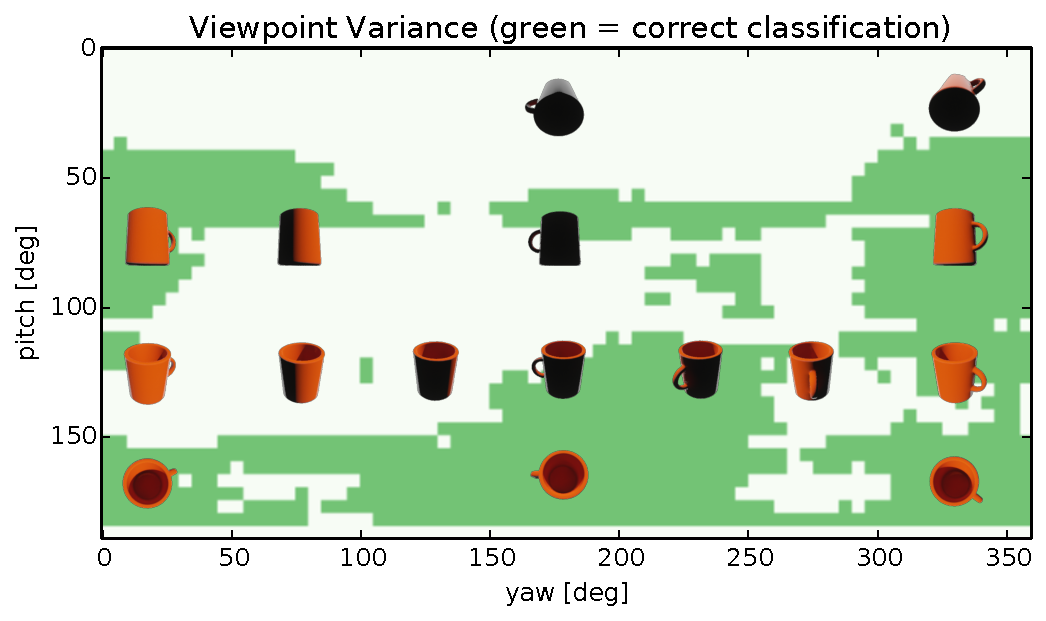
\includegraphics[width=\linewidth]{object_recognition.pdf}
    \caption{Simulated viewpoint-dependency test for the \texttt{vgg\_s} convolutional network \cite{Chatfield14} on a coffee mug object. Successful recognition (green) requires the mug handle to be clearly visible and the object to be well-illuminated.}
    \label{fig:obj-recognition}
\end{figure}


\section{DISCUSSION} \label{sec:discussion}

The most difficult and time consuming aspect of using high-fidelity simulation is creating the scene in the first place. Scenes are built of 3d models and textures, which are first time consuming to create, and then take even more time to arrange in the scene. The more realistic a scene is required to be, the longer both of these stages take. The creation of high quality 3D models and scenes is the speciality of a professional 3D artist, so if a particular problem requires large or realistic scene it may be necessary to hire a 3D artist to construct it. It can also be extremely difficult to maintain a consistent scale throughout the scene. Examination of our scene in Figure \ref{fig:street-scene-overview} will reveal a myriad of scale flaws, note for instance the height of the houses relative to the width of the road.

However, once a particular simulation has been created, it can be used to generate arbitrary amounts of image data. Once we had constructed the street scene and the tools set up, actually capturing each dataset can be specified programatically and takes relatively little time. Indeed, when we initially created the  datasets used to test the place recognition algorithms above, we tested orientation change at $30\degree$ and $15\degree$ only. However, after observing the way matching performance falls off with angle in Figure \ref{fig:sad-results-stacked}, we were able to very easily add tests for $5\degree$ and $10\degree$ orientation changes as well. The very fact that we can exactly repeat a movement through a scene with a precise orientation change is a powerful advantage of high-fidelity simulation.

It can in some sense be too easy to capture data. Since capturing additional data is often simply a matter of adding a new modifier to a path, increasing a sample range or decreasing a sample increment, it can be very easy to generate too much data. For instance, it may be tempting to sample a street scene such as ours at every offset up to 4m either side in 1m increments, and at each location take all vertical and horizontal changes up to $30\degree$ in $5\degree$ intervals. This is relatively simple to specify, but when multiplied out, produces $9 \times 13 \times 13 = 1521$ images per forward step down the path. The path we used with a step distance of 1m as well requires 612 forward steps, for a total therefore of 1965132 images. When capturing datasets ourselves, we averaged about 6 frames per second, so collecting all this data would take approximately 91 hours. It's easy to see how tweaking any of the specified numbers could multiply this number even further.

Rather than sampling densely with a large initial dataset, we recommend initial testing be done relatively sparsely over the test domain, and then using the initial results to choose a second round of test values. For instance, given the distribution for vertical orientation change in Figure \ref{fig:sad-results-stacked}, it makes more sense to generate new test data at $2.5\degree$ and at $7.5\degree$ than at $25\degree$. In the future, it should be possible to automate this iterative testing, automatically choosing new test datasets based on the results of previous testing.

It is also important to note that the difficulty of a particular change to the simulation can be non-intuitive. For instance, it is very easy in the simulation to change the location or orientation of an object or the camera; or to change the base colour of a flat-coloured object. For this reason, it was very easy for us to add additional variations on the camera path, since this simply changes the camera's location and orientation. On the other hand, changing the lighting is simple manually, but for good quality lighting a lot of data needs to be recalculated, which takes a lot of time and is not designed to be triggered programatically. As such, it takes longer to generate data across different times of day, and it would be more time-consuming for us to test at an additional time of day.

\section{CONCLUSIONS AND FUTURE WORK} \label{sec:conclusion}

In this paper we investigated the use of photo-realistic gaming engine simulation tool to address important challenges in robotic vision: that
experiments cannot  be repeated, that algorithms cannot be quantitatively compared, and that for object recognition the lack of labelled training and test
is a bottleneck for training deep networks.
The simulation allows us to create high realistic images from an arbitrary camera or cameras in a complex 3-dimensional world in which lighting and atmospheric
conditions can be set at will.
We  showed how we can systematically evaluate some standard robotic vision algorithms (robust place recognition and visual SLAM) in ways which have not
been previously possible.  These algorithms are broadly representive of the classes of image-based and feature-based methods.
We also showed how we can synthetically generate a large number of images to evaluate a deep network for object recognition.

We have only just begun to scratch the surface of this new approach to robotic vision.
So far our paths through the environment are set manually rather than being driven by a robotic vision algorithm.
Integrating the game engine into the ROS environment would simplify this, allowing us to run a robotic vision algorithm in a manner analagous to a 
hardware-in-the-loop simulator, its output commands the camera pose in the simulator and the rendered image becomes its input.
The fidelity of the simulation approach needs to be tested on a wider variety of common vision algorithms.
Creating complex 3D worlds is time consuming and we are investigating modern 3D reconstruction techniques to create a first draft of a simulated world. It should also be possible to procedurally generate many parts of the environment, establishing rules for the generation of roads, cities, and other environments allowing variations to be produced quickly. Finally, many assets need only be created once, and a wider community using simulation and sharing work should reduce the initial costs of setting up a simulation.

%from camera to simulation
%There remains a significant amount of applications that we have not yet explored. At this time, we have not successfully tested interaction between robot control code and high-fidelity simulation, further work is required on the code interfaces that make this possible. With further investigation, it should be possible to create full simulators for computer vision code including control code that interacts with the simulated world. This opens up the advantages of high-fidelity simulation to all computer vision algorithms, rather than only to passive algorithms.
%
%This paper has focused on using simulation to test and analyse computer vision algorithms, but the generation of image data can also be used to train learning algorithms, such as deep-learning neural nets. Interestingly, it should be possible to apply the iterative testing approach outlined here to network training, alternating between generating new test data to fill holes in the performance graph and generating new training data to correct areas of poor performance, with a reduced risk of over-training.
%%
%The key problem with using high-fidelity simulation is that generating simulation environments is too costly. There are a number of different ways that this can be made easier. Firstly, it is often desirable for simulation environments to mirror a real-world environment in some way, and so it should be possible to use modern 3D reconstruction techniques to lay the groundwork for a simulation environment. It should also be possible to procedurally generate more about the environment, establishing rules for the generation of roads, cities, and other environments allowing variations to be produced quickly. Finally, many assets need only be created, and a wider community using simulation and sharing work should reduce the initial costs of setting up a simulation.
%=======
%\subsection{Future Work}
%
%There remains a significant amount of applications that we have not yet explored. At this time, we have not successfully tested interaction between robot control code and high-fidelity simulation, further work is required on the code interfaces that make this possible. With further investigation, it should be possible to create full simulators for computer vision code including control code that interacts with the simulated world. This opens up the advantages of high-fidelity simulation to all computer vision algorithms, rather than only to passive algorithms.
%
%This paper has focused on using simulation to test and analyse computer vision algorithms, but the generation of image data can also be used to train learning algorithms, such as deep-learning neural nets. Interestingly, it should be possible to apply the iterative testing approach outlined here to network training, alternating between generating new test data to fill holes in the performance graph and generating new training data to correct areas of poor performance, with a reduced risk of over-training.
%
%The key problem with using high-fidelity simulation is that generating simulation environments is too costly. There are a number of different ways that this can be made easier. Firstly, it is often desirable for simulation environments to mirror a real-world environment in some way, and so it should be possible to use modern 3D reconstruction techniques to lay the groundwork for a simulation environment. It should also be possible to procedurally generate more about the environment, establishing rules for the generation of roads, cities, and other environments allowing variations to be produced quickly. Finally, many assets need only be created, and a wider community using simulation and sharing work should reduce the initial costs of setting up a simulation.

\addtolength{\textheight}{-12cm}   % This command serves to balance the column lengths
                                  % on the last page of the document manually. It shortens
                                  % the textheight of the last page by a suitable amount.
                                  % This command does not take effect until the next page
                                  % so it should come on the page before the last. Make
                                  % sure that you do not shorten the textheight too much.

%%%%%%%%%%%%%%%%%%%%%%%%%%%%%%%%%%%%%%%%%%%%%%%%%%%%%%%%%%%%%%%%%%%%%%%%%%%%%%%%



%%%%%%%%%%%%%%%%%%%%%%%%%%%%%%%%%%%%%%%%%%%%%%%%%%%%%%%%%%%%%%%%%%%%%%%%%%%%%%%%



%%%%%%%%%%%%%%%%%%%%%%%%%%%%%%%%%%%%%%%%%%%%%%%%%%%%%%%%%%%%%%%%%%%%%%%%%%%%%%%%
\section*{APPENDIX}

Appendixes should appear before the acknowledgment.

\section*{ACKNOWLEDGMENT}

% Who should I thank here? The institute? thanking a co-author doesn't seem right. Epic Games, since it's their program I'm using?

% The preferred spelling of the word "acknowledgment" in America is without an "e" after the "g". Avoid the stilted expression, "One of us (R. B. G.) thanks . . ."  Instead, try "R. B. G. thanks". Put sponsor acknowledgments in the unnumbered footnote on the first page.



%%%%%%%%%%%%%%%%%%%%%%%%%%%%%%%%%%%%%%%%%%%%%%%%%%%%%%%%%%%%%%%%%%%%%%%%%%%%%%%%


\bibliographystyle{plain}
\bibliography{john-bibliography,sourav-visual-SLAM,HFSinVision}  



\end{document}
